\documentclass{ctexart}

% 导言区
\usepackage[colorlinks,linkcolor=blue,bookmarksopen=true,bookmarksnumbered=true,citecolor=blue]{hyperref}             % 目录点击跳转

% \url 链接换行 参考https://liam.page/2017/05/17/help-the-url-command-from-hyperref-to-break-at-line-wrapping-point/
\makeatletter
\def\UrlAlphabet{%
	\do\a\do\b\do\c\do\d\do\e\do\f\do\g\do\h\do\i\do\j%
	\do\k\do\l\do\m\do\n\do\o\do\p\do\q\do\r\do\s\do\t%
	\do\u\do\v\do\w\do\x\do\y\do\z\do\A\do\B\do\C\do\D%
	\do\E\do\F\do\G\do\H\do\I\do\J\do\K\do\L\do\M\do\N%
	\do\O\do\P\do\Q\do\R\do\S\do\T\do\U\do\V\do\W\do\X%
	\do\Y\do\Z}
\def\UrlDigits{\do\1\do\2\do\3\do\4\do\5\do\6\do\7\do\8\do\9\do\0}
\g@addto@macro{\UrlBreaks}{\UrlOrds}
\g@addto@macro{\UrlBreaks}{\UrlAlphabet}
\g@addto@macro{\UrlBreaks}{\UrlDigits}
\makeatother

\usepackage[]{physics}
\usepackage[]{amsmath}
\usepackage{cite}
\usepackage[colorlinks,linkcolor=blue]{hyperref}
\usepackage{siunitx}
\usepackage{graphicx}
\usepackage{subfigure}
\usepackage{float}
\usepackage[]{epigraph}
\usepackage{xeCJKfntef}
\usepackage[most]{tcolorbox}
\xeCJKsetup{underdot/symbol={\normalfont^^b7}}
\newcommand{\dotemph}[1]{\CJKunderdot{#1}}
\usepackage{geometry}
\geometry{left=2.0cm,right=2.0cm,top=2.5cm,bottom=2.5cm}
\linespread{1.25}% 修改行间距


\newcommand\subtitle[1]{\rightline{\small #1}} 


\setlength{\parindent}{4em}
\title{暗物质及其探测手段简介\\ \subtitle{——ATIC探测项目初探}  } % 添加标题
\author{郑卜凡\quad2021302022016}                     % 添加作者
\date{\today}                             %最后更新日期


\begin{document}
    \maketitle              %制作封面
    \begin{abstract}
        简略的论述了暗物质研究的历史发展和现状,并且从天文学和粒子物理两个方面出发介绍暗物质,较详细的说明了其存在的证据以及目前的探测手段,特别是南极的高空气球ATIC探测项目。
    \end{abstract}
    \tableofcontents        %制作目录
	
	\newpage
	\section{绪论}
	\setlength{\epigraphwidth}{.7\textwidth}
	\epigraph{最能说明科学内在统一性的莫过于将探索宇宙最大物体,即宇宙学,和探索宇宙最小物体,即粒子物理学,结合正在一起所进行的研究。}{E.W.Kolb}
	“物质的基本组成单元是什么?”这个问题可以追溯到两千多年前德谟克利克提出\dotemph{原子}的概念。目前人类已经得到的最精确的答案是粒子物理标准模型(见下图\ref{fig:1}),但是这一定不是最终答案,量子场论中无处不在的无穷大迫使人们引入\dotemph{重整化}来解决,这也使得人们意识到目前的理论也只是个低能有效理论,只是终极理论的一个低能标近似。\cite{AZ}
	
	\begin{figure}[h]
		\centering
		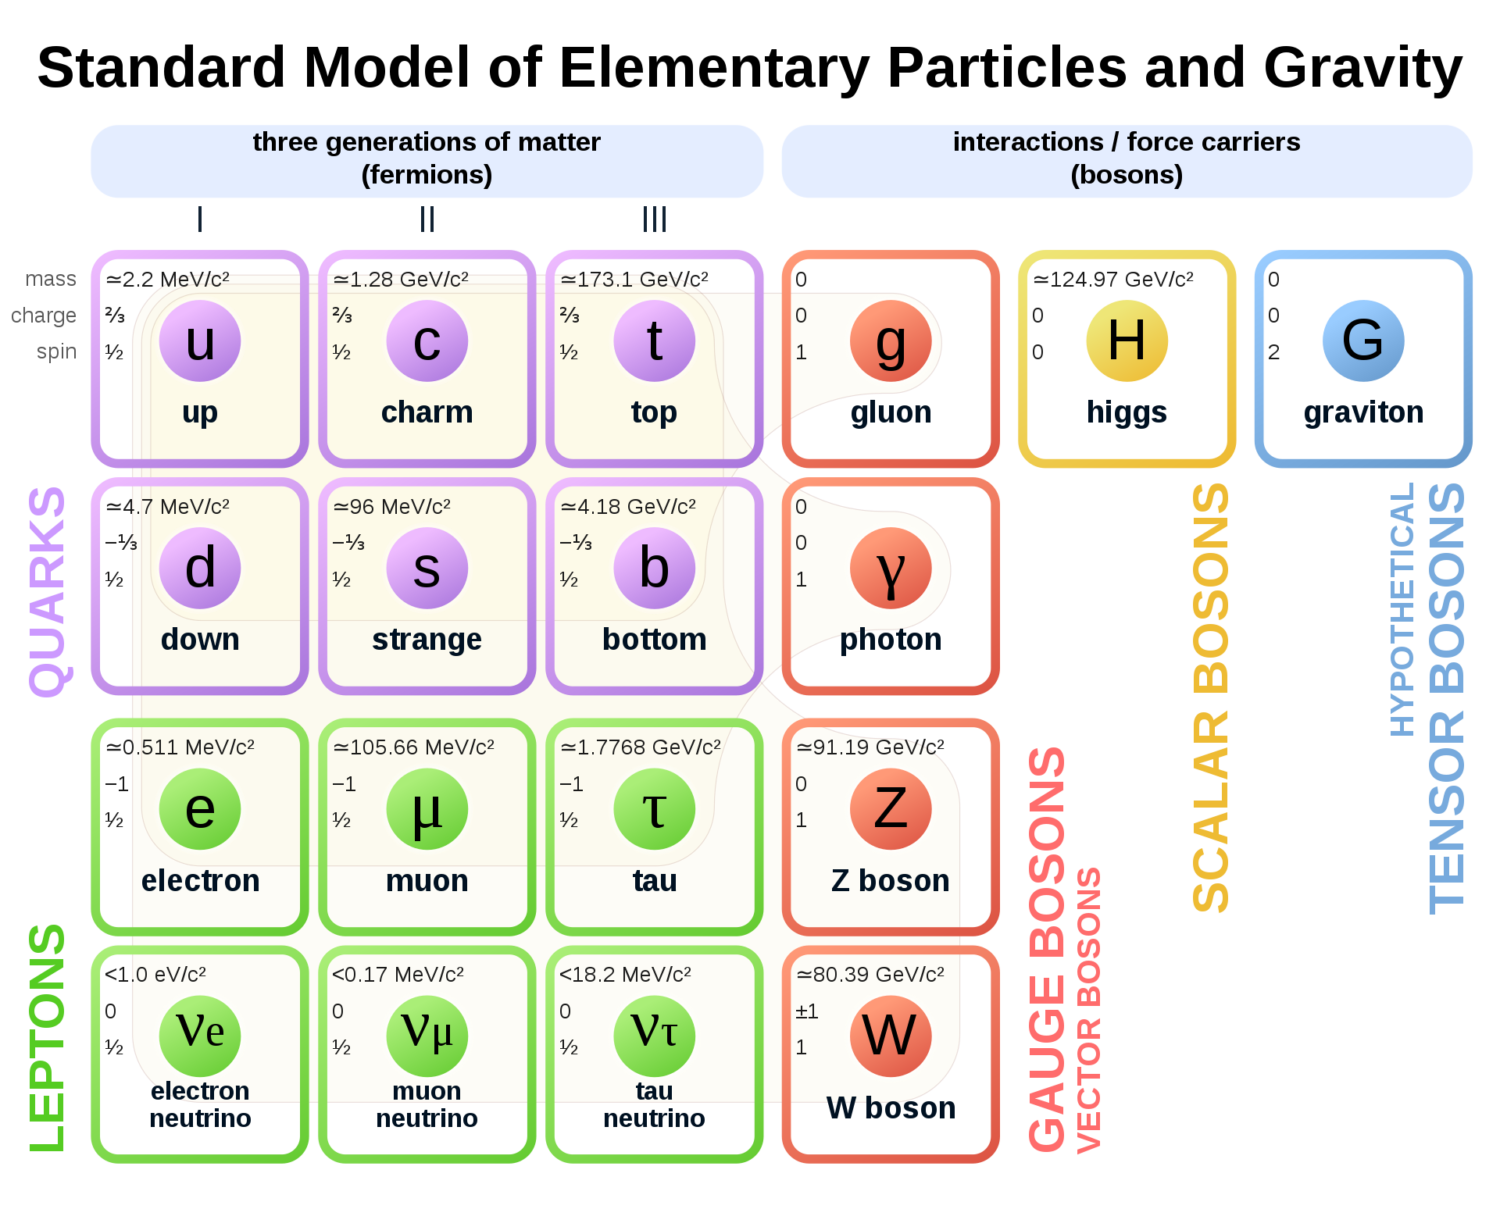
\includegraphics[width=0.618\linewidth]{figs/Standard_Model_of_Elementary_Particles.png}
		\label{fig:1}
		\caption{粒子物理标准模型}
	\end{figure}
	
	另一方面,标准模型并不完美,理论中出现的多达19个参数必须由实验确定,中微子质量的存在性问题\footnote{当然可以通过略微修改理论来引入中微子质量项,但是这也会使得标准模型本身看起来相当不自然。\cite{PFS}}、强CP问题、夸克禁闭问题等等都预示着一些超出标准模型的物理现象,其中一个一人注目的问题就是\textbf{暗物质}谜团。
	
	暗物质最早的存在证据都起源于上世纪初对星系以及星系团的引力效应的观测,观测结果与已知的引力理论相矛盾,要么是引力理论在星系尺度下已经不成立需要修改,要么就是引力理论没问题,还有一些看不见的物质的影响我们没有考虑进来,也就是所谓的暗物质。目前基于天文学的一系列观测告诉我们\footnote{我们将在后面详细介绍这些观测}暗物质理论是必要的,甚至现今宇宙中绝大部分都起源于暗物质(见下图\ref{fig:2})。但是粒子物理学家并不满足于唯象的解释,而是去通过实验探究暗物质究竟是怎样一种超出标准模型的粒子。很遗憾,我们对暗物质所知还是甚少,只知道它们不能是些什么:
	\begin{enumerate}
		\item[$\bullet$] 它们不能是重子物质,不带电荷与色荷;
		\item[$\bullet$] 它们不能由标准模型粒子组成;
		\item[$\bullet$] 它们不参与电磁相互作用,所以不发光也不吸收光,所以我们看不见;
		\item[$\bullet$] 它们确实参与引力相互作用,暗物质的引力效应在宇宙中无处不在。
	\end{enumerate}
	\begin{figure}[h]
		\centering
		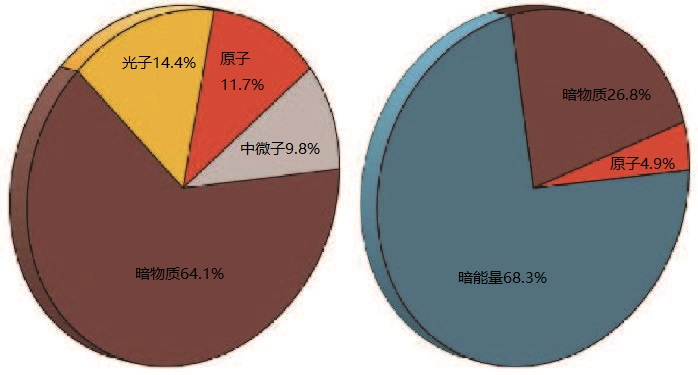
\includegraphics[width = 0.7\linewidth]{figs/dark_matter.jpg}
		\label{fig:2}
		\caption{宇宙中的暗物质组分图,左侧是宇宙初期,右侧是现今宇宙。图源来自《大英百科全书》}
	\end{figure}
	尽管目前来看我们对暗物质所知甚少,还是可以在粒子物理的一些框架下研究暗物质,并且已经有一些包含暗物质可能候选者的理论模型。目前,暗物质研究正处于实验驱动阶段。由大量的已经完成,正在进行或者正在建造中的实验来寻找暗物质粒子。这些实验必然会如以太说驱动广义相对论产生般引发一场巨大的物理学革命!
	
	最后提一下本文的写作结构,本文是读书报告,主要是记录了解暗物质所学习的一些课本或者是论文,所以\dotemph{基本没有原创之处},所有论断都可以在本文后面的参考文献中找到,不过文中必然出现了不少本人自己对论文本身的理解,若有不当,还请指教\footnote{\href{mailto: whuzbf@qq.com}{Email:whuzbf@qq.com}}。
		
	由于文中不可避免的会使用一些定量计算进行论证,所以本文先简略的介绍了一下广义相对论和宇宙学,然后以此为基础重点论述暗物质存在的天文学证据,这也与暗物质研究发展的历史进程相符;之后再从粒子物理方面出发介绍暗物质可能的候选者,最后再用比较长的篇幅论述现今暗物质探测的实验手段,尤其是ATIC项目。
	
	\section{广义相对论与宇宙学回顾}
	注意,我们这里的介绍是相当简略的,想进一步学习的读者可以阅读\cite{GR1}\cite{GR2}。
	
	首先本文选取$c=\hbar=1$的自然单位制,并且选取平直空间中的\textit{Minkovski}度规号差为$-2$,即$(+---)$约定,当然为了不给自己找麻烦,\textit{Einstein}求和约定贯穿本文始终。
	
	在广义相对论中,空间度规用对称的协变和逆变张量表示,分别是$g_{\mu\nu}$和$g^{\mu\nu}$,它们起到升降指标的作用,二者之间的关系为:
	\begin{equation}
		g^{\mu\sigma}g_{\sigma\nu}=\delta^\mu_\nu
	\end{equation}

	狭义相对论中我们考虑的坐标变换是\textit{Lorentz}变换$\Lambda^\mu_{\;\nu}$,而广义相对论中我们更多考虑一般的非线性坐标变换。在坐标变换$x\to x^\prime$下满足下面的变换性质的量称为\dotemph{张量}:
	\begin{equation}
		V^{\mu\cdots}_{\nu\dots}\to V^{\prime\mu\cdots}_{\nu\dots}=\frac{\partial x^{\prime\mu}}{\partial x^\lambda}\cdots\frac{\partial x^\sigma }{\partial x^{\prime \nu}}V^{\lambda\cdots}_{\sigma\dots}
	\end{equation}
	上述张量的协变导数定义为:
	\begin{equation}
		V^{\mu\cdots}_{\nu\dots;\lambda}=\frac{\partial }{\partial x^\lambda}V^{\mu\cdots}_{\nu\dots}+\Gamma^\mu_{\lambda\sigma}V^{\sigma\cdots}_{\nu\dots}+\cdots-\Gamma^\sigma_{\nu\lambda}V^{\mu\cdots}_{\sigma\dots}-\cdots
	\end{equation}
	其中$\gamma^\lambda_{\mu\nu}$叫克氏符号或者仿射联络,由下式给出:
	\begin{equation}
		\Gamma^\lambda_{\mu\nu}=\frac{1}{2}g^{\lambda\sigma}\left(\partial_\mu g_{\nu\sigma}+\partial_\nu g_{\mu\sigma}-\partial_\sigma g_{\mu\nu}\right)
	\end{equation}
	其中$\partial_{\mu}\equiv \frac{\partial }{\partial x^\mu}$.
	
	对于在平直时空中已经得到的各种公式,到狭义相对论中我们只需要将导数换成相应的协变导数就好,比如电荷守恒连续性方程:
	\begin{equation}
		\partial_\mu J^\mu=0\to J^\mu_{\, ; \nu}=0
	\end{equation}
	在平直时空中的自由粒子不受力,运动方程为:
	\begin{equation}
		\dv[2]{xi^\mu}{\tau}=0
	\end{equation}
	其中$\tau$是粒子的固有时,也可使用世界线长等作为参量。$xi^\mu$理解为局部惯性系下的广义坐标,在局部惯性系下度规张量就是平直时空中的\textit{Minkovski}度规$\eta_{\mu\nu}$,一般的度规张量为:
	\begin{equation}
		g_{\alpha\beta}(x^\mu)\equiv\eta_{\mu\nu}\pv{\xi^\mu}{x^\alpha}\pv{\xi^\nu}{x^\beta}
	\end{equation}
	上式可以理解为广义相对论中度规张量的定义,在此定义下,世界线长是标量:
	\begin{equation}
		ds^2=\eta_{\mu\nu}\dd \xi^{\mu}\dd \xi^{\nu}=g_{\alpha\beta}\dd x^\alpha \dd x^\beta
	\end{equation}
	
	利用\dotemph{等效原理},立即得到广义相对论中的测地线方程:
	\begin{equation}
		\boxed{
		\dv[2]{x^\mu}{\tau}+\Gamma^\lambda_{\alpha\beta}\dv{x^\alpha}{\tau}	\dv{x^\beta}{\tau}	=0
	}
	\end{equation}
	还有几个几何学参数,首先是\textit{Riemann}曲率张量:\footnote{这里不同的书又有不同的习惯,\textit{Riemman}曲率张量是根据$A_{\beta;\mu\nu}-A_{\beta;\nu\mu}=R^\lambda_{\;\beta\mu\nu}A_\lambda$定义的(揭示了协变导数不对易),有的文献和这里相差一个符号,需要注意。}
	\begin{equation}
		R^{\lambda}_{\;\beta\mu\nu}\equiv\pdv{\Gamma^\lambda_{\nu\beta}}{x^\mu}-\pdv{\Gamma^{\lambda}_{\mu\beta}}{x^\nu}+\Gamma^\alpha_{\nu\beta}\Gamma^\lambda_{\mu\alpha}-\Gamma^{\alpha}_{\mu\beta}\Gamma^\lambda_{\nu\alpha}
	\end{equation}
	分别作一次缩并和两次缩并后得到\textit{Ricci}张量和\textit{Ricci}标量:
	\begin{equation}
		R_{\alpha\beta}=R^\lambda_{\;\alpha\lambda\beta}\qquad \qquad R\equiv \Tr R_{\alpha\beta}=R^\alpha_{\;\alpha}=g^{\alpha\beta}R_{\alpha\beta}
	\end{equation}
	\textit{Riemman}张量有如下对称性:
	\begin{equation}
		R_{\alpha\beta\mu\nu}=-R_{\alpha\beta\nu\mu}=-R_{\beta\alpha\mu\nu}=R_{\mu\nu\alpha\beta},\quad	R_{\alpha\beta\mu\nu}+R_{\alpha\mu\nu\beta}+R_{\alpha\nu\beta\mu}=0
	\end{equation}
	还有下面的{\itshape Bianchi}恒等式成立:
	\begin{equation}
		R_{\alpha\beta\mu\nu;\lambda}+R_{\alpha\beta\nu\lambda;\mu}+R_{\alpha\beta\lambda\mu;\nu}=0
	\end{equation}
	\textit{Einstein}场方程为:
	\begin{equation}
		\label{GREQ}
		\boxed{
		R_{\mu\nu}-\frac{1}{2}g_{\mu\nu}R-{\color{red} \Lambda g_{\mu\nu}}=8\pi G T_{\mu\nu}
	}
	\end{equation}
	
	方程左边是几何量,右边是能动张量是物质量,$G$是万有引力常量,$\Lambda$是宇宙学常数,Einstein当初引入这一项是为了得到静态的宇宙学解,被其称为“一生中最大的错误”,然而现在发现这一项对于宇宙演化是必要的,可以解释为暗物质和暗能量项,后面将详细讨论。
	
	能动量张量可以利用下式进行计算:
	\begin{equation}
		T^{\mu\nu}=\sum\frac{p_n^\mu p_n^\nu}{E_n^2}\delta\left(\mathbf{x}-\mathbf{x}_n\right)
	\end{equation}

	其中一类非常重要的模型是相对论性理想流体模型,在局部惯性系下\footnote{或者后面$\S 3.4$将会提到的共动参照系}流体相对静止,相应的能动量张量为:
	\begin{equation}
		T^{\mu\nu}=\mqty(\dmat{\varepsilon,P,P,P})
	\end{equation}
	$P$是压强,$\varepsilon$是对应的能量。一般的参考系下能动量张量为:
	\begin{equation}
		\label{eq:17}
		T^{\mu\nu}=(\varepsilon+P)U^\mu U^\nu-Pg^{\mu\nu}
	\end{equation}
	其中$U^\mu$是四维速度。对于一般的在壳粒子,由于$E^2=c^2p^2+m^2c^4$,有如下等式成立:
	\begin{equation}
		\label{eq:18}
		0\leq P\leq \frac{1}{3}\varepsilon
	\end{equation}

	具体的$P$和$\varepsilon$之间的关系称为\dotemph{状态方程},与物质本身的性质有关,例如对于星际尘埃(非相对论性的物质),上面不等式取左极限,对于辐射和极端相对论性物质(光子),上面不等式取右极限。更多其它物质的状态方程可以查阅文献\cite{Linder1997FirstPO}。
	
	\section{天文学观测证据}
	本节主要从历史的脉络出发介绍暗物质存在的天文学证据。首先我们以列表\footnote{这个列表是对J.Primack 2009 年所作题为 \textit{A Brief History of Dark Matter}报告的总结,遗憾的是我未能再次找到其报告的视频网址。}的形式简要概述一下暗物质天文观测的历史进程,这里不打算详细介绍这些观测的意义和物理原理,想了解更详细的历史细节可以查阅这篇比较新的综述文章\cite{RevModPhys.90.045002}。
	
	暗物质早期历史:
	\begin{enumerate}
		\item[$\bullet$] 1922-Kepteyn:猜测银河系星系盘存在所谓暗物质;
		\item[$\bullet$] 1933,1937-Zwiky:后发星系团暗物质;
		\item[$\bullet$] 1937-Smith:室女座星系团“大质量的星云物质”;
		\item[$\bullet$] 1937-Holmberg:来自于几对星系的质量,$5\times 10^{11}M_{\odot}$;
		\item[$\bullet$] 1939-Babcock观测到M31星系\footnote{这个星系是离银河系星系最近的仙女座螺旋星系}的上升旋转曲线;
		\item[$\bullet$] 1940s-许多观测证实了星系团的大$\sigma V$结果;
		\item[$\bullet$] 1957-van de Hulst:发现M31的高HI旋转曲线;
		\item[$\bullet$] 1959-Kahn \& Woltjer:MWy-M31交汇处$\to M_{\text{LocalGroup}}=1.8\times 10^{12} M_\odot$;
		\item[$\bullet$] 1970-Robin \& Ford:M31平坦光学旋转曲线;
		\item[$\bullet$] 1973-Ostriker \& Peebles:晕稳定了星系盘;
		\item[$\bullet$] 1974-Einasto, Kaasik \& Saar; Ostriker, Peebles \& Yahil::总结了星系M/L随半径增长的证据;
		\item[$\bullet$] 1975,1978-Roberts,Bosma:HI扩展的平坦旋转曲线;
		\item[$\bullet$] 1978-Mathews:X射线揭示了室女座星系团的巨大质量;
		\item[$\bullet$] 1979-Faber \& Gallagher:提出暗物质存在的令人信服的证据;
		\item[$\bullet$] 1980-\textit{Now}:大多数天文学家相信暗物质存在于星系和星系团周围。
	\end{enumerate}
	\subsection{星系旋转曲线}
	这是最早的暗物质存在的天文观测证据,也是最容易理解的,提供了大量非重子物质存在的证据。
	
	考虑一个简化的模型,能更清晰的说明问题,考虑两种球对称的质量分布,$M(r)$表示在$r$半径球内的总质量:\footnote{$\theta$是阶跃函数,定义为$\theta(x)=\begin{cases}
			0,& x<0\\
			1,& x>0
		\end{cases}$}
	\begin{align}
		\label{caseA} M_A(r)&=M_T\left(\frac{r}{R}\right)^3\theta(R-r)+M_T\theta(r-R)\\
		\label{caseB} M_B(r)&=M_T\left(\frac{r}{R}\right)^3\theta(R-r)+M_T\left(\frac{r}{R}\right)\theta(r-R)\\
	\end{align}

	\ref{caseA}就是通常能想到的星系中物质分布,物质分布全部集中在一个半径为$R$的球体中,而\ref{caseB}就表明在球体外还有逐渐减少的物质分布,现在主流解释为“暗物质晕”分布在星系周围。
	
	依据这两种物质分布可以求得对应的星系旋转曲线,即对于旋转星系距离系中心$r$处的旋转速度,满足方程:
	\begin{equation}
		\frac{v(r)^2}{r}=G\frac{M(r)}{r^2}
	\end{equation}
	下图\ref{fig:3}给出了两种情况下的星系旋转曲线大致形状:
	\begin{figure}[h]
		\centering
		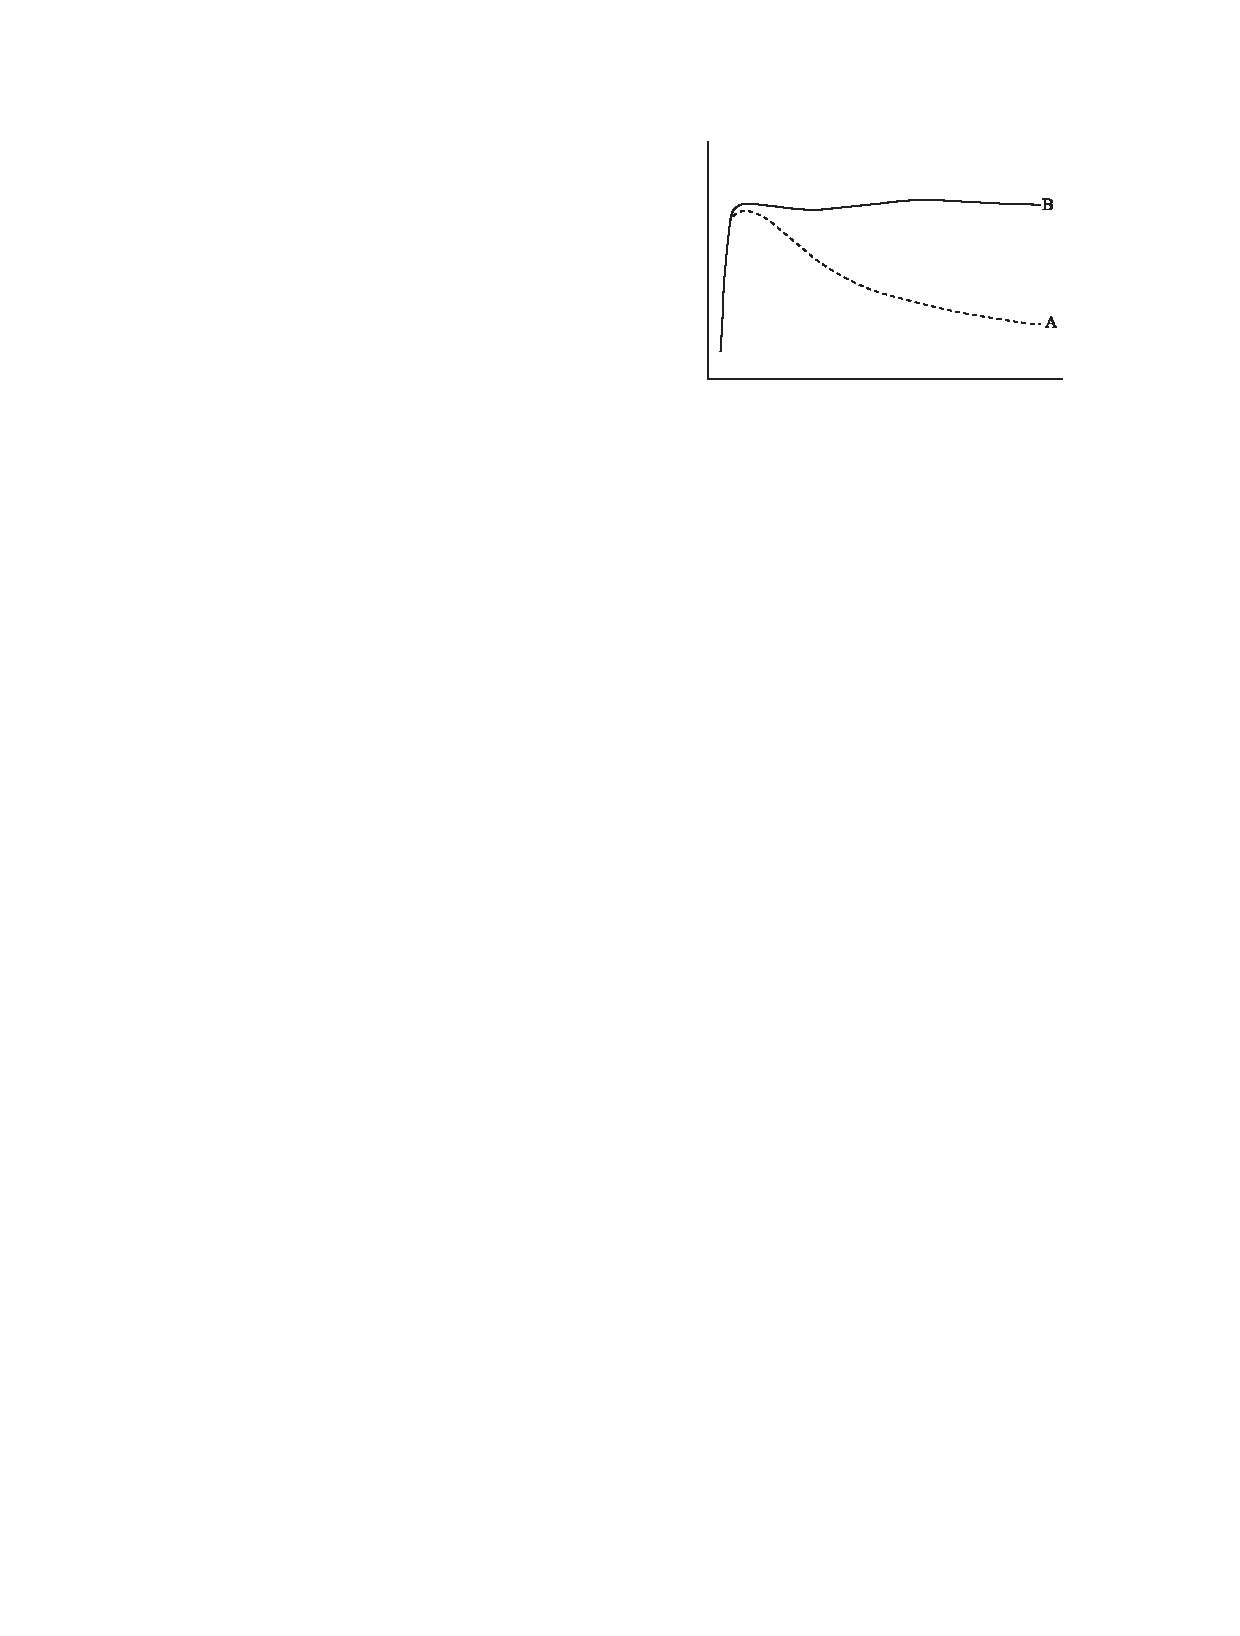
\includegraphics[width=.618\linewidth]{figs/fig3.pdf}
		\label{fig:3}
		\caption{两种质量分布情况下的星系旋转曲线,纵轴为旋转速度,横轴为距离$r$}
	\end{figure}
	
	有意思的是,观测到的旋转曲线是$B$,而观测到的星系物质分布是$A$,显然这意味着还有一些\dotemph{我们看不见的物质},便命名为暗物质。事实上,在考虑$A$物质分布的时候,不难计算出在$r_{esc}=2R$处所有物质的旋转速度都大于逃逸速度,实际观测发现超过这一半径许多倍仍有许多恒星存在,所以必须要引入所谓“暗物质”来产生足够的引力从而不至于让星系自转解体。
	
	\subsection{星系团的质量}
	正如恒星会在引力的作用下聚集形成星系,星系之间也会在由于引力而结团形成更大的星系团结构。通过观察星系团中的各个星系的亮度和运动情况,人们可以推算出整个星系团的质量,这里主要有两种方法:
	\begin{enumerate}
		\item[$\bullet$] 根据星系团中星系的数量和整体发光情况去反推星系团的质量,这被称为“光度质量”。
		\item[$\bullet$] 测量星系团中大量星系的运动速度,根据速度的离散程度,可以通过引力理论去计算星系团的质量,由这种方法得到的质量被称为“动力学质量”。
	\end{enumerate}
	
	如果星系团中的大多数物质是发光的,那么这两种质量应当不相上下。然而在三十年代,天文学家Zwicky和Smith却发现了一件不可思议的事:某些星系团的光度质量实际上远小于其动力学质量。这反映出了一个难以置信的事实:宇宙中发光物质或者说可见物质的总量可能要远少于不发光的物质。这些不发光的物质不参与电磁相互作用,没有任何电磁信号,人们只能通过其庞大的引力效应去感受它们。这就是暗物质最初的观测证据。不过,由于当时人们对物质的微观模型了解甚少,且对星系团系统的稳定性存在争议,所以没有暗物质给予足够的重视。
	
	\subsection{引力透镜效应与子弹星系团}
	\textit{Einstein}的广义相对论预言在大质量星体附近测地线是弯曲的,光线在经过这些天体周围时路径会发生偏折,就像经过了一个透镜一样。所以人们可以根据对引力透镜效应的观测结果反推星系团的质量分布。
	
	2006年,哈勃望远镜对子弹星系团\footnote{国际编号1E0657-56}的质量分布观测结果为暗物质的存在提供了迄今为止之最好的证据\cite{Clowe_2006}。下图\ref{fig:5}中粉红色部分是由X射线信号反映出的可见物质的分布,蓝色部分则是由引力透镜效应反推出的总的质量分布,可以看到二者是不重合的。这说明可见物质并不能主导星系团的质量,它们只占星系团总物质的一小部分,星系团的大部分质量是由不可见的暗物质提供的。
	\begin{figure}[h]
		\centering
		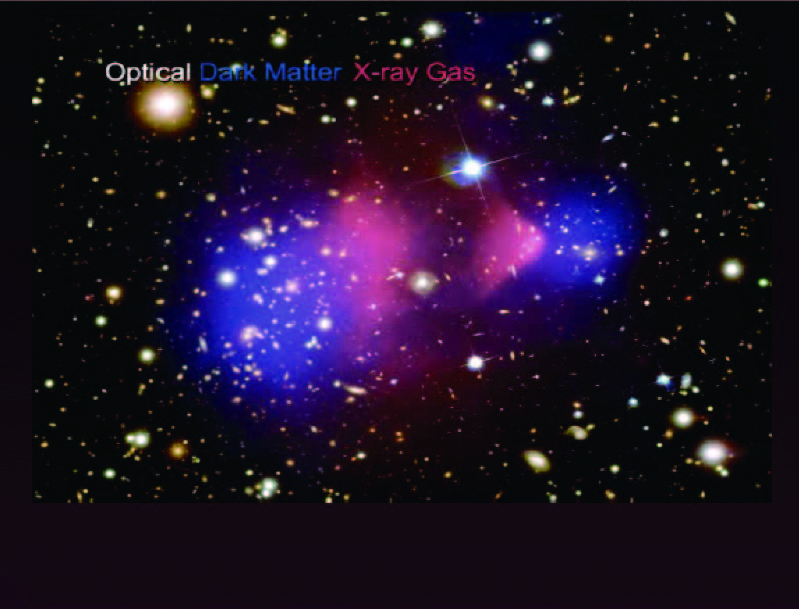
\includegraphics[width=.6\linewidth]{figs/fig5.jpg}
		\label{fig:5}
		\caption[]{可见图中物质中心和引力中心明显不重合}
	\end{figure}
	而且这个观测结果用引力的修正理论是难以解释的,另外对其它星系团之间的碰撞观测,例如MACSJ0025.4-1222\cite{Brada2008RevealingTP},也显示了可见物质中心和引力中心的明显偏移,而且在星系团的碰撞中,暗物质并未明显减速也限制了暗物质之间以及暗物质和物质之间的相互作用之强度。
	
	\subsection{暗物质与加速膨胀的宇宙}
	首先我们来简要看一下方程\ref{GREQ}中宇宙学常数这一项带来了什么,我们将这一项移到右边从而解释为物质项:
	\begin{equation}
		R_{\mu\nu}-\frac{1}{2}g_{\mu\nu}R=8\pi G\left(T_{\mu\nu}+T_{\mu\nu}^\Lambda\right)\quad T_{\mu\nu}^\Lambda\frac{\Lambda}{8\pi G}g_{\mu\nu}
	\end{equation}
	与理想流体的能动张量表达式\ref{eq:17}对比不难发现:
	\begin{equation}
		\epsilon_\Lambda=\frac{\Lambda}{8\pi G},\qquad P_\Lambda=-\frac{\Lambda}{8\pi G} 
	\end{equation}

	显然这里大于零的$\Lambda$会产生负压强与辐射和通常物质产生的引力相抗衡,这也是\textit{Einstein}引入宇宙学项来构造静态宇宙模型的原因。而且上面的状态方程明显是与不等式\ref{eq:18}相悖的,这意味一种超出现今物理学标准模型的物质等待着被发现。
	
	我们再来看一下弱场近似下的引力场,真空中,也即不存在重子物质的空间中,引力场方程变为:
	\begin{equation}
		R_{\mu\nu}+\Lambda g_{\mu\nu}=0
	\end{equation}
	这个方程有球对称的解,也即所谓的\textit{Schwarzchild-de Sitter}度规:
	\begin{equation}
		g_{\mu\nu}=\mqty(\dmat{A(r),-B(r),-r^2,-r^2\sin^2{\theta}})
	\end{equation}
	其中:
	\begin{equation*}
		A(r)=1-\frac{2GM}{r}-\frac{1}{3}\Lambda r^2\qquad B(r)=\frac{1}{A(r)}
	\end{equation*}
	
	在弱场近似下,广义相对论退化为牛顿万有引力理论,引力由引力势描述$\mathbf{F}=-\nabla \Phi$,与度规之间的关系为:\footnote{这里很容易想到$c\to\infty$近似下只有度规的时间分量产生贡献,本文强调的是概念而不是具体的计算,更详细的计算可以在文献\cite{GR1}的第四章中找到。}
	\begin{equation}
		g_{00}\approx 1+2\Phi
	\end{equation}

	$\Lambda=0$时$\Phi\approx -\frac{GM}{r}$,退化到经典引力理论,引力势满足Poisson方程$\nabla^2\Phi=4\pi G\rho(\mathbf{r})$;$\Lambda\neq 0$时$\Phi\approx -\frac{GM}{r}-\frac{1}{6}\Lambda r^2$,会带来排斥势抵消通常的重子物质的影响,与之前的分析一致。
	
	接下来将目光转向宇宙学,整个宇宙虽然说在星系团尺度上存在物质涨落,但是就整个宇宙的大尺度而言宇宙是均匀的,对宇宙微波背景辐射(CMB)的观测也说明了这一点。日心说和地心说看来都不正确,宇宙并不存在一个绝对的中心,不过就研究方便而言,把我们自己选取为宇宙中心是个明智的方法,在这之上我们还可以选取一个特殊的参照系,随宇宙一起膨胀,所有物质都相对于这个参照系静止,我们称之为\dotemph{共动参考系}。
	\begin{tcolorbox}[colback=red!5!white,colframe=red!75!black,title=宇宙学原理]
		在足够大的尺度上,宇宙是均匀且各向同性的。
	\end{tcolorbox}
	依据这一原理我们可以导出描述宇宙大尺度的共动参考系下的\textbf{F}riedmann-\textbf{R}obertson-\textbf{W}alker(FRW)度规:\cite{Weinberg}
	\begin{equation}
		\boxed{
			\dd[2] s=\dd[2] t-a(t)^2\left[\frac{\dd[2]r}{1-\kappa r^2}+r^2\dd[2]\theta+r^2\sin^2\theta\dd[2]\phi \right]
	}
	\end{equation}
	其中$a(t)>1$称为标度因子\footnote{多说一句,标度因子本身不是可观测量,其比值才是。},$\kappa$是曲率常数,可以取下面三个数值,对应三种不同的宇宙几何结构:
	\begin{equation}
		\kappa =\begin{cases}
			+1,&\text{球面,正曲率,封闭宇宙}\\
			-1,&\text{超球面,负曲率,开放宇宙}\\
			0,&\text{欧几里得,无曲率,平坦宇宙}
		\end{cases}
	\end{equation}
	目前的天文观测支持$\kappa=0$的情况。
	
	在共动参考系下离我们距离为$L$的星系\footnote{前文说过,将我们自己视为宇宙中心}与我们之间的\dotemph{固有距离}可以如下简单计算为:
	\begin{equation}
		D(t)=\int_0^L\dd r\sqrt{g_{rr}}=\begin{cases}
			a(t)L,&\kappa=0\\
			a(t)\sin^{-1}L,&\kappa=+1\\
			a(t)\sinh^{-1}L,&\kappa=-1\\
		\end{cases}
	\end{equation}
	进而可以定义下面的\textit{Hubble}系数:
	\begin{equation}
		H(t)\equiv\frac{\dot{D}}{D}=\frac{\dot{a}}{a}
	\end{equation}
	在现在我们所处的时间$t_0$,天文观测得到\textit{Hubble}常数$H_0$的值为\footnote{$\operatorname{pc}$是天文学单位——秒差距}:
	\begin{equation}
		H_0\approx 70\operatorname{km}\cdot\operatorname{s}^{-1}\cdot\operatorname{Mpc}^{-1}=3\times10^{-18}\operatorname{s}
	\end{equation}
	这意味着我们的宇宙正在膨胀!
	
	现在我们将FRW度规作为\textit{Einstein}场方程的宇宙学解代入,并利用理想流体模型,得到下面两个独立的方程,具体推导见一般的宇宙学书籍:
	\begin{align}
		\label{eq:33} -\frac{\ddot{a}}{a}+\Lambda&=4\pi G\left(\varepsilon+3P\right)\\
		\label{eq:34} \frac{\ddot{a}a+2\dot{a}^2+2\kappa}{a^2}-\Lambda&=4\pi G\left(\varepsilon-P\right)
	\end{align}
	
	其中$\varepsilon$和$P$分别是寻常物质的能量和压强,而且根据宇宙学原理,在共动参考系中它们只和时间有关。
	
	从\ref{eq:33}和\ref{eq:34}可以看出唯一使得宇宙膨胀加速,也即$\ddot{a}>0$的项是$\Lambda$,这两个方程还可以解出关于$\varepsilon$和$P$的形式:
	\begin{align}
		\frac{8\pi G}{3}\varepsilon&=\frac{\dot a ^2}{a^2}+\frac{\kappa}{a^2}-\frac{1}{3}\Lambda\\
		\label{eq:36}-8\pi G P&=\frac{2\ddot{a}}{a}+\frac{\dot{a}^2}{a^2}+\frac{\kappa}{a^2}-\Lambda
	\end{align}

	定义\dotemph{减速}参量\footnote{为啥是减速而不是加速是个历史原因,因为之前天文学家们坚信宇宙是在减速膨胀}:
	\begin{equation}
		q\equiv -\frac{\ddot a a}{a^2}=-\frac{\ddot a}{H^2 a}
	\end{equation}

	将$\kappa=0$的式\ref{eq:36}代入$q$的定义式并且注意到目前宇宙中可观测到的物质以及辐射产生的压强相比于$\varepsilon$而言可以忽略不计,即$P\approx 0$。我们得到\footnote{所有下标0都告诉我们代表物理参量在当前宇宙年龄取值}:
	\begin{equation}
		q_0=\frac{1}{2}\left(1-\frac{\Lambda}{H_0^2}\right)
	\end{equation}

	$\Lambda=0$对应有$q_0=0.5>0$,宇宙确实由于物质的引力在减速膨胀,但目前的观测\cite{Riess_1998}\cite{Perlmutter_1999}告诉我们$q_0\approx-0.5<0$,也就是说宇宙是在\dotemph{加速膨胀}的!这一项工作被授予了2011年度的Nobel物理学奖\footnote{\href{https://www.nobelprize.org/prizes/physics/2011/summary/}{https://www.nobelprize.org/prizes/physics/2011/summary/}}。这也告诉我们必须存在适当的$\lambda\sim 10^{-52}$使得宇宙加速膨胀,这可以解释为暗物质的作用\footnote{当然也有理论认为其来源于量子场论中的真空能,但是解释的并不完美。}。
	\subsection{宇宙大尺度结构}
	\begin{figure}[h]
		\centering
		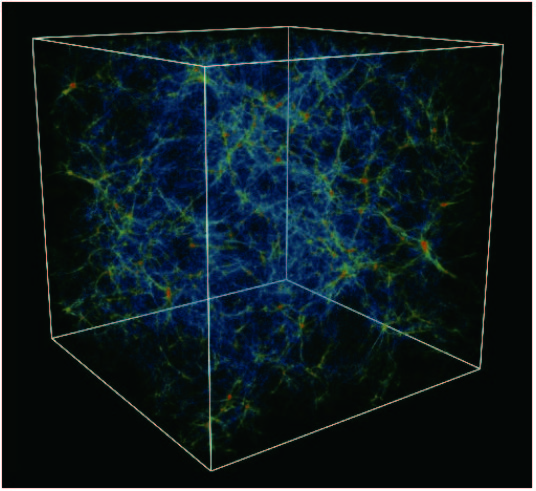
\includegraphics[width=.5\linewidth]{figs/fig4.jpg}
		\label{fig:4}
		\caption[]{宇宙的大尺度结构模拟示意图}
	\end{figure}
	
	上图\ref{fig:4}揭示了宇宙的大尺度结构,可以发现由细丝和空洞构成,细丝的交界处表示物质的高度聚集区域,那里会发现大量的星系团,而空洞则是宇宙中平均密度很低的区域。在不断膨胀的宇宙模型中,固定在空间纤维上的任意两个点之间的距离也在不断增大。如果没有某种力来吸住它们,它们之间将永远分离。而单纯靠物质之间的引力是不够的,需要引入暗物质,对宇宙大尺度结构的模拟和观测更重要的意义是确定暗物质的种类。
	
	如果暗物质由重的\footnote{可以达到GeV甚至Tev量级。}、低速、非相对论粒子构成,这被称为冷暗物质(CDM)。冷暗物质会使物质聚集到小的区域,因此宇宙中会弥漫着大量较小的矮星系。反之,如果暗物质是由具有弱相互作用的相对论性粒子组成的,质量在eV量级甚至更轻,则称为热暗物质(HDM)。\footnote{当然介于它们之间还有所谓的温暗物质(WDM)模型,质量在KeV量级或者重一点。}
	
	两种不同的暗物质模型预言了不同的宇宙大尺度结构,通过计算机模拟可以得到下面的图\ref{fig:6}:
	\begin{figure}[h]
		\centering
		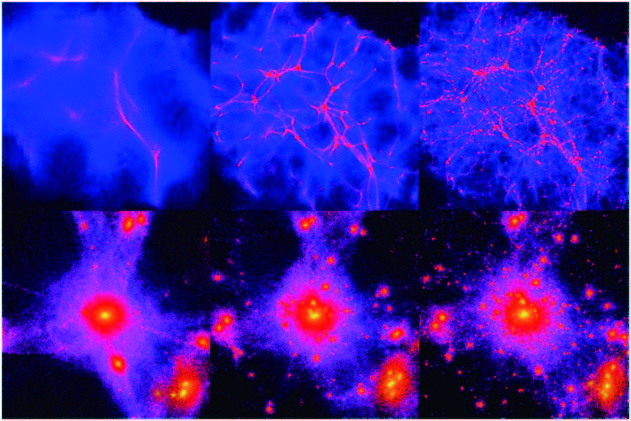
\includegraphics[width=.618\linewidth]{figs/fig6.jpg}
		\label{fig:6}
		\caption{对两种暗物质模型的宇宙大尺度结构数值模拟,上面对应CDM,下面对应HDM}
	\end{figure}
	与图\ref{fig:5}对比可明显发现,现今的天文观测支持CDM暗物质模型。
	
	\section{暗物质的候选者}
	在介绍暗物质的可能组成之前,先来总结一下暗物质应有的性质:
	\begin{enumerate}
		\item[$\bullet$] 不参与电磁相互作用和强相互作用,否则会有电磁信号或与原子核强烈作用。
		\item[$\bullet$] 必须是稳定的,因为要经过宇宙138亿年的演化遗留至今。
		\item[$\bullet$] 必须在早期宇宙中产生,因为在CMB中有暗物质的信号。
		\item[$\bullet$] 暗物质在星系结构开始形成之时是非相对论性运动的,即动能远小于其质量对应的静能。这样才能让宇宙形成今天这样的网状大尺度结构。(CDM)
	\end{enumerate}
	
	基于这些事实,粒子物理学家为暗物质构建了许多合理的模型,绝大部分都来自于超出标准模型的新理论。比较有名的是以下几类:弱作用大质量粒子(WIMP)、轴子、惰性中微子、超大质量粒子\footnote{它还有一个非常中二的名字:哥斯拉级暗粒子。}。接下来分别介绍一下。
	\subsection{WIMP}
	\textbf{W}eakly \textbf{I}nteracting \textbf{M}assive \textbf{P}article,即弱相互作用大质量粒子,
	这是一类基本粒子模型的统称,指的是质量在GeV~TeV数量级,相互作用强度与标准模型的弱相互作用差不多的粒子。这类粒子如果存在的话,它们会在宇宙大爆炸之初大量产生。然后在宇宙的温度降低至WIMP粒子的质量能标之后,它们会快速地相互湮灭,最终剩余一部分遗留至今成为暗物质。
	
	WIMP型暗物质可以从许多超出标准模型的理论中得到,它们的相互作用截面适中,且质量在TeV数量级以下也容易被下一代的粒子对撞机检验,因此得到了广泛的关注。最热门的WIMP型暗物质候选者是最轻的超对称粒子\footnote{超弦理论中的最轻\textit{Kaluza–Klein}粒子}。超对称是人们为了解决标准模型的规范等级问题、大统一问题而引入的一种玻色子与费米子之间的对称性,认为每一个玻色子都对应一个费米子作为超对称伙伴,反之亦然。因此超对称理论中会引入许多超对称粒子,其中最轻的超对称粒子不会衰变到其他超对称粒子,所以足够稳定可以充当暗物质的角色。
	
	\subsection{轴子}
	粒子物理标准模型存在一个疑难问题,那就是——为什么强相互作用的CP宇称是守恒的?在理论上完全可以存在强相互作用的CP对称性破坏,但实际上却没有发现这种事情。为了解决这一问题,物理学家们构建了一种新的粒子物理模型——Peccei-Quinn模型,里面引入了一种叫做轴子的粒子。轴子的质量非常小,远不到eV的数量级,但它可以从极早期宇宙的\underline{QCD相变}\footnote{水在自然界中在不同温度压强下有固液气三种状态,这是水分子在电磁相互作用层面上的相变现象,如果把温度加热到万亿摄氏度,约为宇宙大爆炸几十微秒后的温度,QCD预言夸克与胶子将摆脱强作用力束缚,从核子中逃离(解禁闭),形成一种由自由夸克与胶子组成的新物质形态,即夸克-胶子等离子体(Quark-Gluon Plasma, QGP)。宇宙冷却过程中必定有QGP到普通强子物质的相变发生,也即QCD相变。}中大量产生,从而充满全宇宙,成为暗物质候选者。\cite{doi:10.1142/S0217751X10048846}\cite{Duffy_2009}
	
	\subsection{惰性中微子$\nu_R$}
	标准模型还有一个疑难问题——为什么中微子的质量那么小?为了解决这一问题,物理学家们提出了一种“跷跷板机制”。也就是,引入某种右手中微子,使它的质量与标准模型的左手中微子相关联。当右手中微子的质量足够大时,左手中微子的质量就会被压得很低\cite[PFS]。这种新引入的右手中微子与标准模型粒子没有直接相互作用,所以被称为惰性中微子,其质量在keV量级(WDM)。
	
	当然也有以其它中微子为中心的理论,比如普通中微子$\nu$,不过其质量如此之小被归类为HDM,目前的天文观测不倾向于这种可能,最多贡献也不会超过几个百分点。
	\subsection{超大质量粒子与超轻矢量粒子}
	指的是质量大于暴胀能标(约$10^{13}$ GeV)的一类粒子。这种粒子如果存在,它会有两种主要的产生途径。第一种是在宇宙暴胀时期通过真空量子涨落产生,这是一种典型的引力量子效应,暗物质是从真空中“凭空”涌现出来的。第二种通过其他热粒子湮灭的“freeze in”机制产生,大体意思就是说宇宙重加热之后有一堆温度极高的热粒子,这些热粒子可以通过与暗物质粒子直接耦合或者通过引力子作为传播子,来把能量传递给暗物质场,激发出暗物质粒子。
	
	超轻矢量粒子是指质量小于eV数量级(超轻)的自旋1(矢量)的暗物质粒子模型。它的产生途径也是在宇宙暴胀时期通过真空量子涨落产生,但与超大质量粒子不同的一点是,超轻矢量粒子在宇宙暴胀时期会经历一种所谓“快子”状态,这会导致它的产生率激增,从而使得质量如此之小的它也可以达到当前所观测到的暗物质总量。
	\subsection{KK粒子}
	KK粒子(Kaluza-Klein)是由同名的物理理论所预言的一种粒子。在量子力学尚未完全建立的1921年,为了统一电磁力和引力,可普查引入了额外维的想法。在很多额外维模型中,平常的3+1维时空被称为膜,它被嵌入在3+δ+1维的被称为bulk的时空中。额外维被卷缩在很小的尺度而感受不到,甚至现在的高能物理实验也远不能探测到,但通过量子效应,额外维会对宇宙产生影响。在很多额外维模型中,标准模型粒子被束缚在膜上,只有引力子可以不受膜的束缚在bulk中传播。而在普遍的额外维模型(UED,universal extra dimensions)中如果额外维很小,所有的场都可以自由地在bulk中传播。
	
	这种理论认为空间有额外的维度并且在每个时空点卷曲起来。KK粒子的质量大约是550到650个质子那么重,它们能够和可见物质发生引力和电磁相互作用,但是由于它们藏在卷曲的额外空间维度里面,所以在太空中看不到它。所幸的是,它能够衰变成所能观测到的粒子。但是现在的大型对撞机实验还没有找到这方面的迹象。
	\subsection{原初黑洞}
	在早期对暗物质的探索中,许多大型天体也被认为是暗物质的候选者产生额外的引力,但是现今的天文观测已经排除了很多此类可能性,这里介绍比较有名的原初黑洞理论。
	
	所谓“原初”,也即在极早期宇宙产生的黑洞,这种黑洞与恒星坍缩成的黑洞非常不同,它不是由天体物理过程演化形成的,而是从极早期宇宙的密度涨落直接形成的。在宇宙诞生的极早期,宇宙暴胀为宇宙带来了原初的密度扰动,如果某些时空区域的密度扰动幅度足够大,那么随着视界扩大它就会包含足够多的物质,直接把这片时空区域坍缩成黑洞,这就是所谓的原初黑洞。
	
	由于霍金辐射效应\footnote{真正去理解霍金辐射效应涉及到量子场论中很深奥的知识,有意思的是在Hawking著名科普书籍《时间简史》中给出了一个比较大众化的解释:真空中会自发产生正反粒子对,它们一般来说会迅速湮灭,所以能量还是守恒的,不过黑洞附近可能某个粒子被吸收,这样剩下的那个粒子就无法湮灭,看起来就像是黑洞向外发射粒子,也即Hawking辐射,从而慢慢蒸发。不过这一解释虽然通俗易懂,但是很大程度上歪曲了Hawking辐射原本的意思。},原初黑洞从诞生后会慢慢蒸发损失质量,因此即使原初黑洞在极早期宇宙中产生,它也不一定能存活到今天。不过,黑洞质量越大蒸发速度越慢,由计算可知质量大于 $10^9$ 吨的原初黑洞经过了138亿年的演化依然可以存活到今天,从而充当暗物质。引力波、引力透镜等实验可以对能够充当全部暗物质的原初黑洞的质量提供较强的限制。目前基本可以确定如果原初黑洞大量存在的话,它的平均质量应在太阳质量以下,并拥有一个较宽的质量分布。未来的空间引力波探测实验,如LISA或我国的太极计划,可以对原初黑洞的参数空间提供更强的限制\footnote{暗物质研究实验总是在做排除法。},进一步检验这种暗物质模型的可行性。
	\section{暗物质的探测实验}
	前面说了这么多天文学上的观测,对于天文学家来说暗物质的存在性已经毋庸置疑了,但是对于粒子物理学家来说,研究暗物质在非引力相互作用下的行为是非常重要的,从而对标准模型进行修正。在现今的理论框架下,暗物质与普通粒子之间可能存在弱相互作用,这也是驱动所有实验进行的根源。而暗物质候选者如此之多,需要靠专门针对某种暗物质模型设计的暗物质探测实验来进行验证,单一的实验是不可能成功的,所以目前正在运行的暗物质探测项目非常多。依据实验环境,大致可以将暗物质探测实验分为三类:深地探测、空间探测和对撞机实验。
	
	\subsection{深地探测}
	由于暗物质与普通物质之间相互作用十分微弱,这不但是对探测器本身灵敏度的一个挑战,另外我们还要尽可能的屏蔽掉本底信号的干扰,其中最显著的就是来自宇宙射线$\mu$子衰变而成的中子。所以简单粗暴的方法就是将实验室建在地底,利用地壳屏蔽干扰信号,目前比较有名的实验有:美国的SuperCDMS实验,欧洲的EDELWEISS实验、XENON实验,以及中国的锦屏(CJPL)实验、PandaX实验等等,详情见下面的地图\ref{fig:7}。
	\begin{figure}[h]
		\centering
		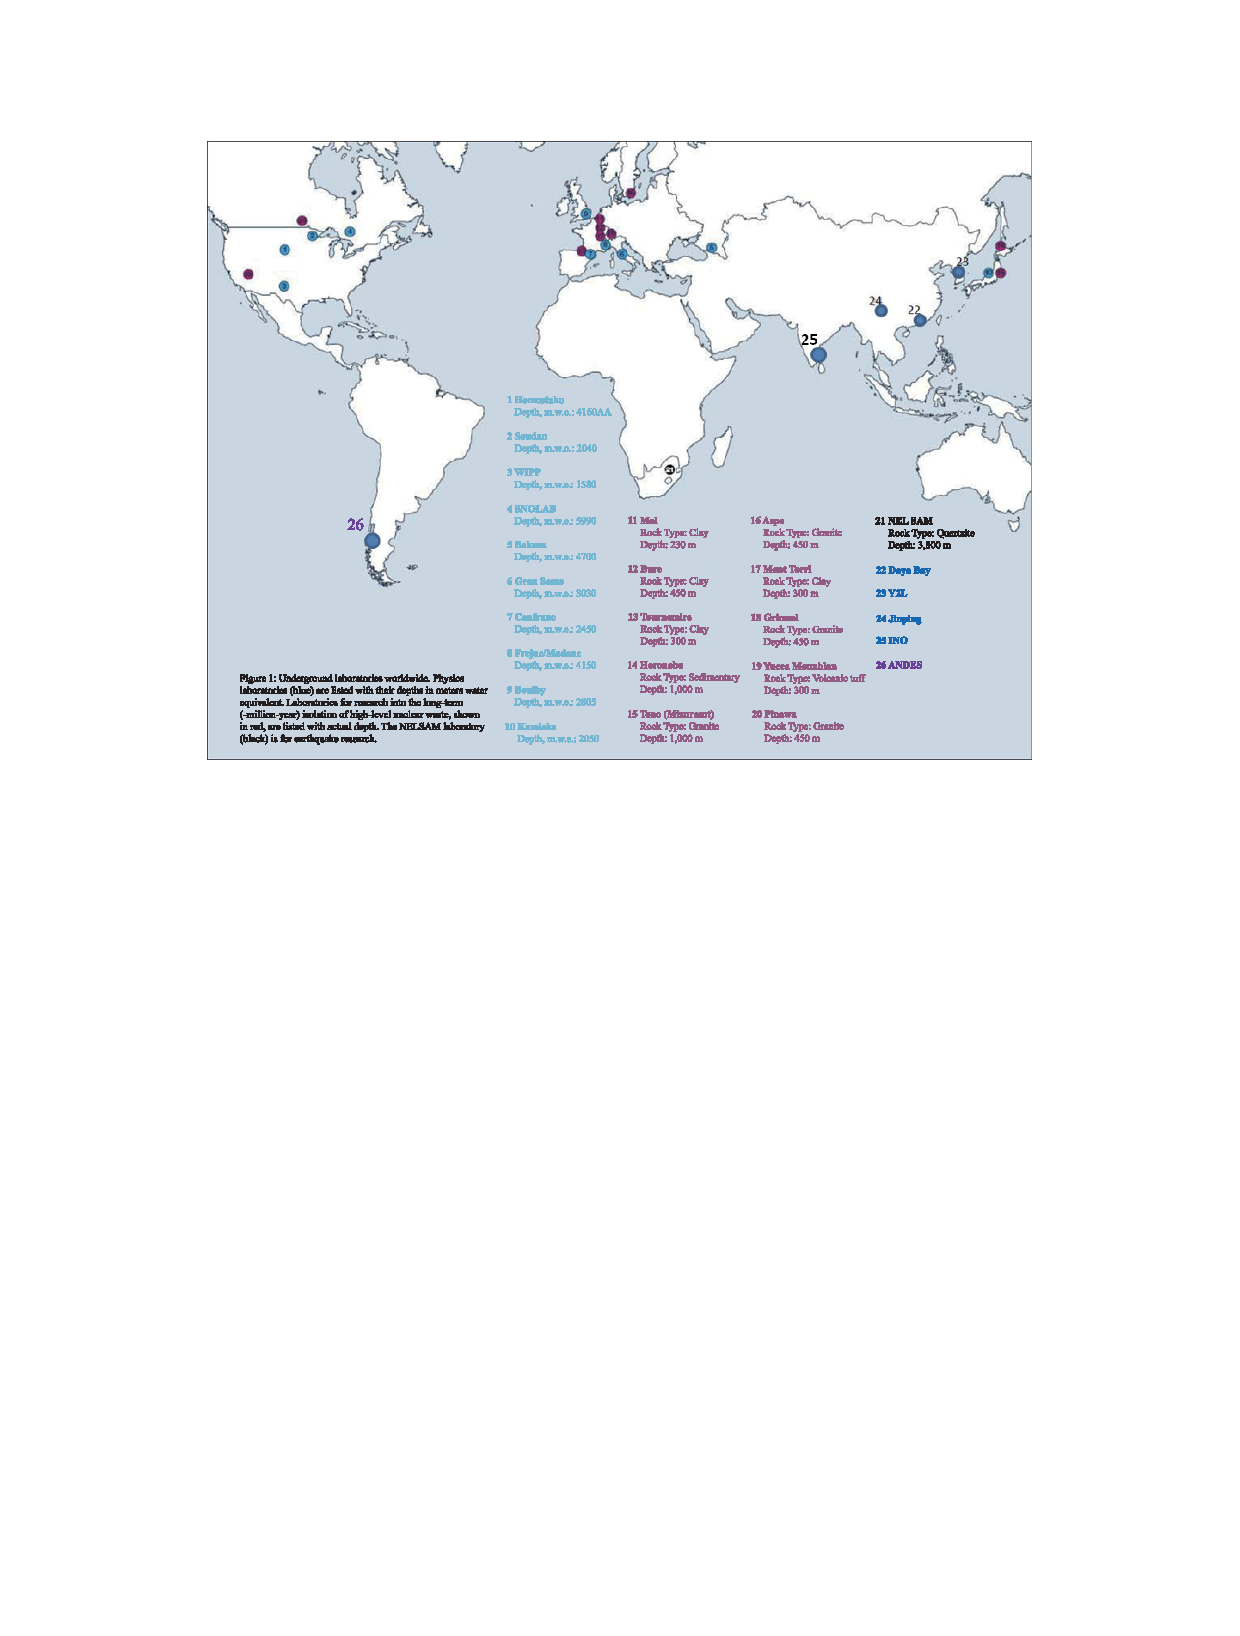
\includegraphics[width=\linewidth]{figs/fig7.pdf}
		\label{fig:7}
		\caption{世界上现在正在运行的暗物质深地实验}
	\end{figure}
	目前的深地实验主要是针对WIMP型暗物质的直接探测。根据暗物质模型,星系的可见物质被引力束缚在一个更重的范围更大的暗物质晕中,地球随着太阳系不断地在星系晕暗物质粒子流中穿梭,一旦暗物质粒子与探测器中的普通物质相互作用,我们就可以通过探测被暗物质敲出来的核子反冲从而确定暗物质的存在,并测量散射截面等物理量与理论预言相比较。
	
	比如中国的PandaX实验(下图\ref{fig:8}\footnote{图源自:\href{http://www.pppi.sdu.edu.cn/info/1041/2937.htm}{粒子物理与粒子辐照教育部重点实验室}}),它的主要实验装置是一个装满了4吨高纯度液氙的容器,在容器的顶部与底部布满了光电探测器。如果有暗物质粒子从外部射入这个探测器,它就有一定概率与氙原子的原子核发生碰撞,从而产生光电信号,被探测器捕捉到。然而,绝大多数的实验至今都没有发现超出本底的信号,也就是说,从统计的角度没有发现暗物质的显著痕迹。
	\begin{figure}[h]
		\centering
		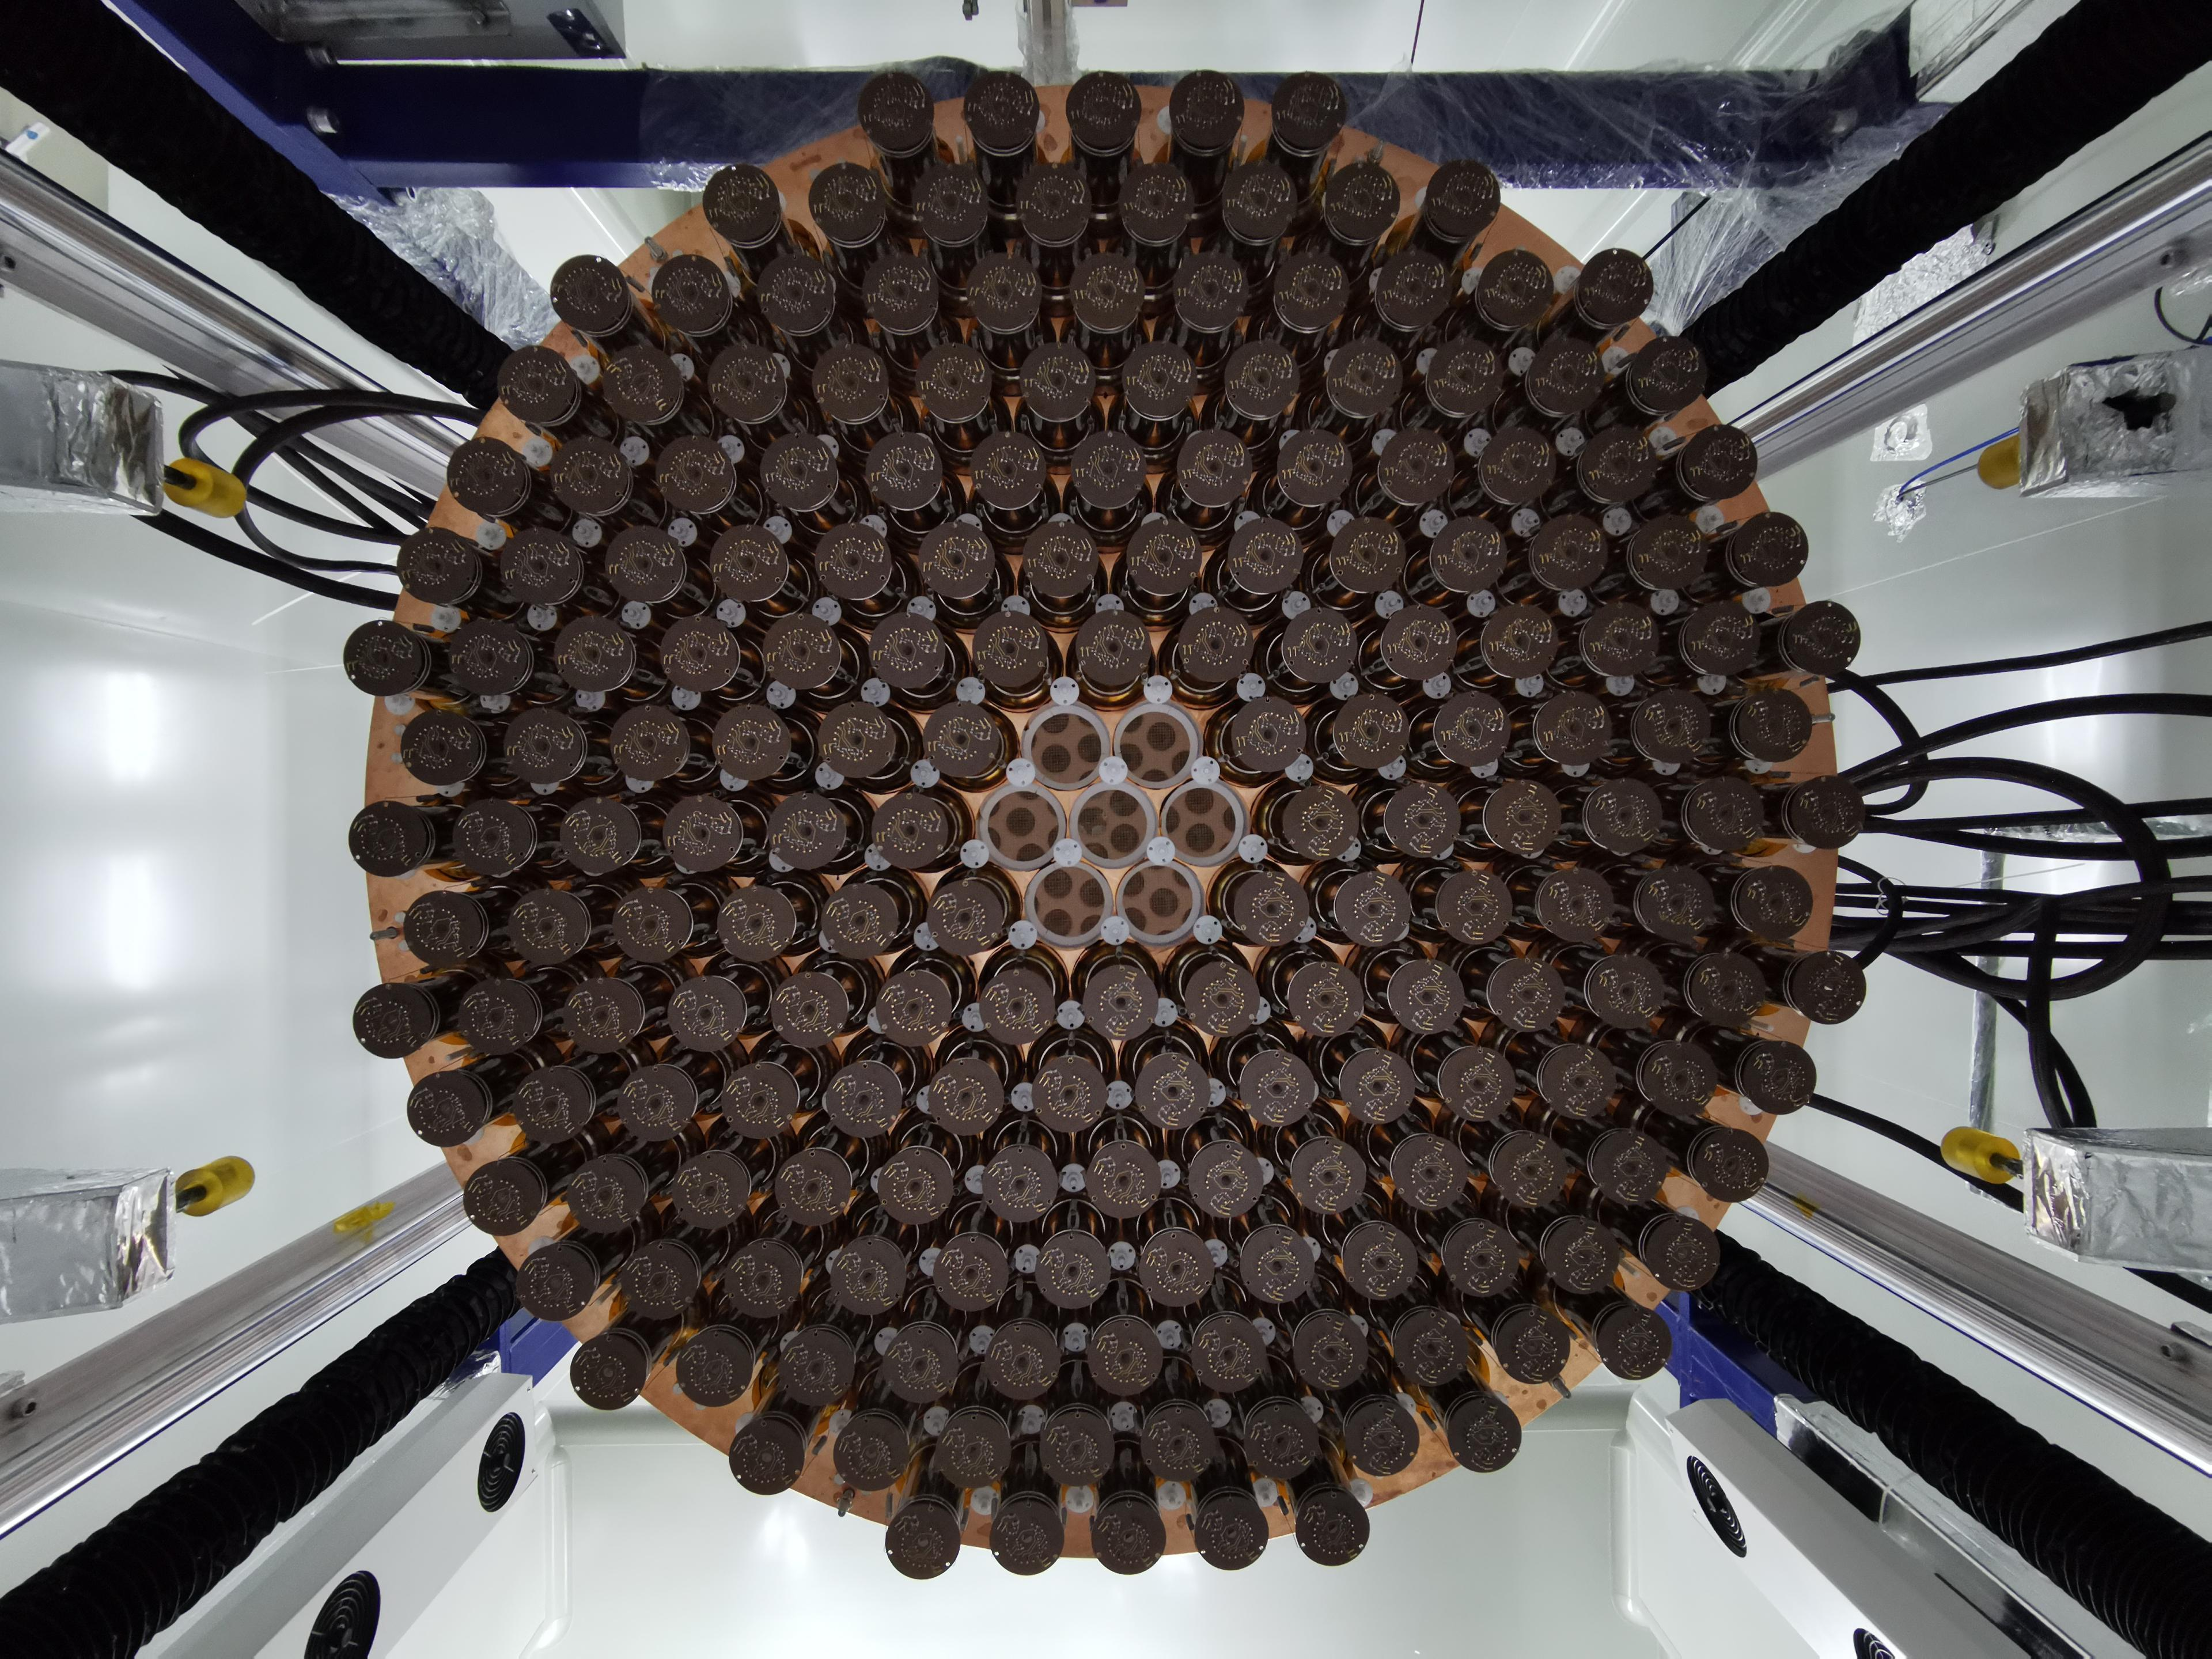
\includegraphics[width=.45\linewidth]{figs/fig8-1.jpg}
		\hspace{.05\linewidth}
		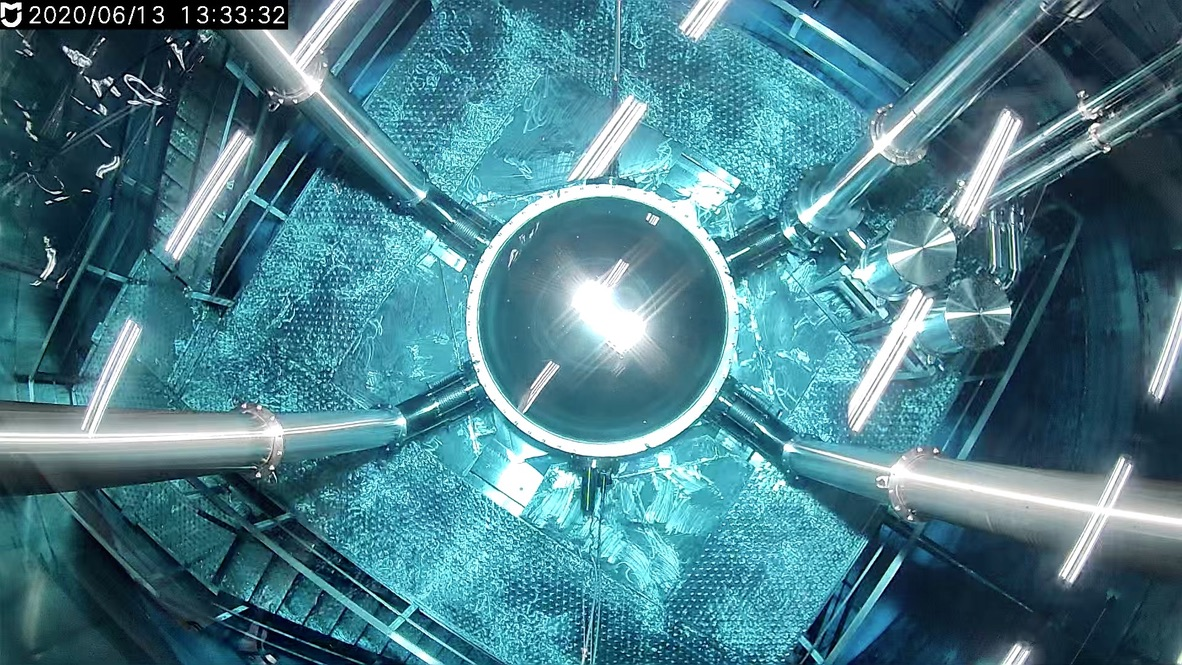
\includegraphics[width=.45\linewidth]{figs/fig8-2.jpg}
		\label{fig:8}
		\caption{中国的PandaX实验}
	\end{figure}
	\subsection{空间实验}
	空间实验和深地实验是对立的两面,空间实验室搭建在绕地卫星上,比较著名的实验包括:国际空间站的AMS实验、美国的Fermi卫星、中国的DAMPE卫星(悟空号)等等。
	
	不过空间实验主要采用的是\dotemph{间接探测}手段,间接探测与直接探测最大的区别就在于其信号可以来源于各种天体,并不局限于太阳系,可以让我们进一步了解暗物质在宇宙中的分布情况。
	
	间接探测通过探测暗物质粒子相互碰撞后产生的看得见的粒子(普通例子),来推测看不见的粒子(暗物质),特别要关注的是反物质信号相对于宇宙线背景的反常,因为反物质本来宇宙中就很稀有。比如丁肇中先生领导的AMS02项目就是通过磁谱仪探测反粒子在磁场中偏转从而测定其动量,观测得到的正电子$e^+$以及反质子$\bar{p}$在高能段下与理论模型相比有明显的\dotemph{超出}现象,不过由于AMS02本身观测能段的限制,目前还无法分辨这个超出来源于暗物质还是特殊天体。
	
	目前我国的悟空号暗物质探测器主要是通过探测伽马射线谱线以及高能电子的能谱来探测暗物质粒子,观测能段在TeV量级,能量分辨率小于$1.5\%$,本地抑制率大于$10^5$,在世界上处于领先阶段\footnote{\href{http://pmo.cas.cn/dampe/}{暗物质粒子探测卫星}}。
	
	\subsection{对撞机产生}
	如果暗物质粒子是在早期宇宙的高温环境中产生的,那么它应该也可以在高能加速器,例如LHC上产生,除非它们只和轻子相互作用。但是遗憾的是,目前人类没有在对撞机上探测到任何有关信号,要么说明暗物质粒子的质量太大,超出了对撞机的最高有效能量;要么质量太小,淹没在了标准模型粒子的背景中;也有可能它们与标准模型粒子的相互作用太弱,以至于产生的数量太少,没有明显的统计信号。
	
	\subsection{其它实验}
	除了上面讲的这些实验,在前面$\S 4$中的讨论中我们还介绍过轴子、惰性中微子等。它们也有对应的探测实验,比如用于探测轴子的ADMX实验,通过探测中微子来判断暗物质的超级神冈(Super-K)\footnote{预计2027年超级神冈将会升级为\href{https://www-sk.icrr.u-tokyo.ac.jp/en/hk/}{顶级神冈(Hyper-K)实验},神冈项目在探测太阳中微子上为日本赢得了两个诺贝尔奖,所以一致在政府的支持下不断升级!}\cite{Super-K}、冰立方(IceCube)\cite{IceCube}实验等。
	
	\hspace*{\fill}
	\noindent\makebox[\linewidth]{\rule{.5\paperwidth}{0.4pt}}
	\hspace*{\fill}
	
	说了这么多实验,但实际上到目前位置人类还没有探测到任何暗物质的信号,或者说观测到了很多反常现象却无法确定是不是由暗物质产生的,在暗物质探测这件事上,人类还有很长的路要走。
	
	\section{ATIC项目}
	\subsection{项目简介}
	1997年,美国宇航局在南极成立了一个名为“ATIC”(\textbf{A}dvanced \textbf{T}hin \textbf{I}onization\textbf{C}alorimeter,先进薄电离量能器)的科考项目,用来观测宇宙线。仪器本身是一个在南极洲上空平流层飞行的气球携带探测设备观测宇宙线的组成,旨在对从氢到铁的原子核进行50GeV到100TeV的宇宙射线元素光谱测量。这些测量结果有望提供有关当今天体粒子物理学中一些最基本问题的信息。
	
	该项目的主要实验装置结构与如下图\ref{fig:8}所示,既然是探测宇宙线,基本想法就是用不同性质的材料做成多层网格结构,不同层对应不同功能根据材料本身性质测量宇宙线的不同组成部分,当宇宙射线打到仪器上时,与材料之间发生相互作用就会被记录下来,网状的结构便会精确记录下宇宙线的径迹,剩下要做的事情就是使用原始数据对宇宙线进行径迹重构,并据此分析宇宙线的组成。
	
	图中最上面那层是使用4480个硅晶单元排列而成的四块平面,通过传感器的宇宙线在废弃区域产生电离,与粒子电荷的平方成正比,所以主要是用于对于宇宙射线所带电荷的精确测量。标注2的的三个平面学名叫“闪烁体描迹仪”(Scintillator Hodoscopes),顾名思义,就是精确的描绘粒子的径迹,主题就是三块由塑料闪烁体\footnote{X射线、CT、核医学放射性核素成像、环境辐射监测、高能射线探测,其原理都是利用光子流作为射线源,射线穿透人体或物质,再从人体或物质中发射出来或射线直接被探测器接收而形成影像。所以探测器系统对射线的接收程度就成为关键的因素之一,而闪烁晶体因其固有的吸收射线辐射发光的特性就成为测量射线能量和强度的良好材料。而塑料闪烁体是有机闪烁物质在塑料中的固容体,一般由基质闪烁物质及移波剂组成。 基质材料多是聚苯乙烯等闪烁物质,移波剂的作用是把闪烁光有效的快速传输及延长。 顺便说一句,塑料闪烁体不是晶体,只是有机闪烁体,可用于快中子、质子、宇宙射线等的探测。}打造而成的平板。再往下走那三块比较厚的板是石墨靶,引起强子相互作用,于是会在最下面的BGO热量仪里产生簇射。热量仪中的能量沉积确定了粒子能量,并提供跟踪信息,所以其也被称作“BGO量能器”,负责宇宙线能量的测量,并通过测量簇射沉积能量的空间分布来进行粒子种类鉴别(区分电子和强子)
	
	\begin{figure}[h]
		\centering
		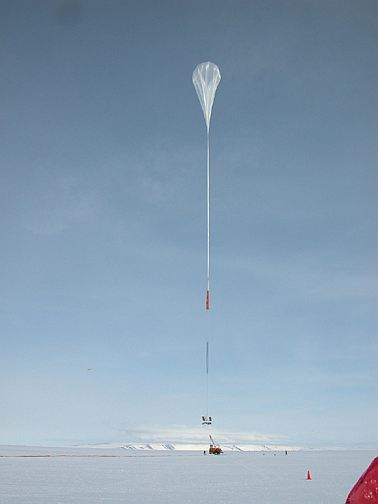
\includegraphics[width=.33\linewidth]{figs/fig9-1.jpg}
		\hspace{.05\linewidth}
		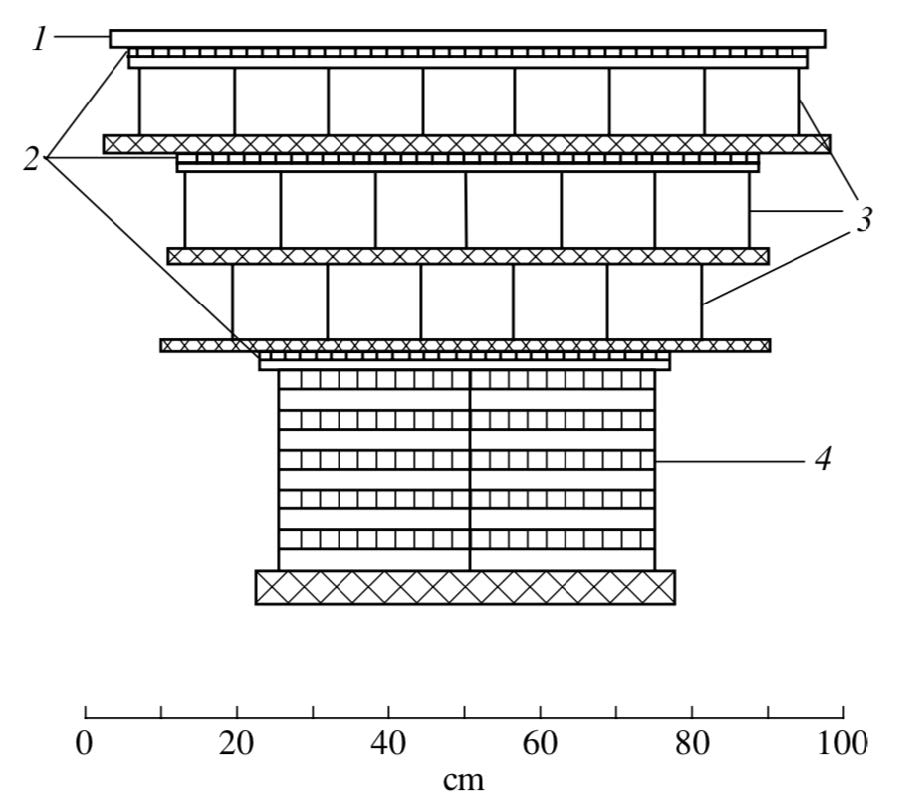
\includegraphics[width=.5\linewidth]{figs/fig9-2.jpg}
		\label{fig:9}
		\caption{ATIC项目装置图,左图为发射时的外观图,右图为实验装置的简化示意图}
	\end{figure}
	
	
	似乎ATIC项目设计之初就是对宇宙线的测量,并不是暗物质观测,不过值得一提的是,其计划提出同年,中国科学家\dotemph{常进}经过反复演算后向该项目首席科学家发邮件建议充分利用ATIC的性能来观测高能电子,因为宇宙线的流量相对于高能电子或是高能$\gamma$光子而言要大得多也更容易观测,故ATIC设计时并没想到去观测高能电子。后来美国科学家经过测试和计算采纳了常进的这一建议,前面我们说过暗物质可能会导致高能电子谱的超出现象,所以这一建议也直接催生了ATIC最有价值的一项发现——宇宙射线正负电子在高能段超出天体物理标准模型。常进先生目前也是我国暗物质探测卫星“悟空号”的首席科学家。\footnote{\href{http://nao.cas.cn/gkjj/zb/xrld/202010/t20201026_5722201.html}{国家天文台——常进}}
	
	\subsection{ATIC与暗物质}
	ATIC对暗物质的测量手段属于间接测量,2008年,报告\cite{RN33}声称利用ATIC项目观测到了宇宙射线中高能电子与标准模型的“超出”现象。在此之前宇宙线探测卫星PAMELA项目其实也观测到过高能正电子谱的“超出”现象,不过ATIC是无法区分正电子和电子的,所以这两次实验相互印证,说明了暗物质的存在性。更加可喜可贺的是,它与暗物质候选者KK粒子\footnote{见$\S 4.5$}相互作用并湮灭成电子-正电子对时的预期信号类型一致。而且峰值的620GeV能量大致是粒子物理理论预期的KK粒子的质量,很好的支持了这一理论模型,但是测量到的信号强度非常高,这是不容易解释的,只能认为我们太阳系正在经过一个非常密集的暗物质团,这显然不是让人满意的解释,也没有其它实验能说明这一点。
	
	但是这仅仅只是一种看似合理的对超出现象的解释,比如脉冲星,类星体这些天体都可能对电子谱产生影响。所以别高兴太早,我们仅仅只是确定了存在异常数据,但是完全无法解释清楚其根源究竟是什么!
	\subsection{对ATIC项目现状的评论}
	从2000年ATIC项目第一期升空到08年的ATIC-4项目完美运行,ATIC项目已经顺利完成了四期宇宙线探测任务,ATIC项目的重点是探测宇宙射线,但其对暗物质的意外发现无疑称为ATIC最重要的科研成果,即使知道现在我们也无法对ATIC所观测到的电子谱超出现象提供确切的物理起源解释,但是这一怪异的现象激起了科学界讨论暗物质的热潮,引起了人们对暗物质实验的兴趣,从这一点上看ATIC项目是非常成功的。其为理论测试和超出标准模型的新物理寻找都提供了机会,对天体物理学家来说,通过ATIC提供的宇宙线观测数据,也能一瞥极端宇宙环境中发生的过程和现象,如超新星、脉冲星等极端天体的性质。
	
	
	\section{总结}
	这篇文章\footnote{本文是粒子物理课程上关于暗物质主题讨论的课程报告,读书笔记类型,本文使用\LaTeX 编写,项目Github地址为:\url{https://github.com/WHUZBF/MyReports/tree/main/粒子物理中期报告}}由于是读书笔记类型,所以很多讨论都可以在文中注明的文献中找到。
	
	虽说选修的是粒子物理课程,不过为了大致能看懂暗物质的一些初级文献,所以用了一个多月时间抽空学习广义相对论和宇宙学相关的极初步内容\footnote{其实就是懂了点基本假设,看得懂几个GR里重要的方程},它们构成了本文前半部分内容,后半部分就是对暗物质专门的讨论了,通过精读暗物质的经典综述文章\cite{RN32},以及历史性综述文章\cite{RevModPhys.90.045002},它们构成了本文$\S3$和$\S4$的内容。
	
	最后就是关于暗物质探测实验方面的内容,这一方面主要是去查阅相关项目组的官方网站,并略读了相关的一些论文(相关的论文在文中都有提及),这构成了本文的$\S 5$,由于ATIC项目是小组选题,所以看了更多关于这个项目的有关资料\footnote{可以浏览宇宙线物理组官网浏览更多信息:\url{https://cosmicray.umd.edu/index.php}},单独写成$\S 6$,这便是本文的全部结构了。
	
	
	
	\nocite{*}
	\bibliographystyle{unsrt} % unsrt 按照引用顺序排序; plain 按照字母顺序排序参考文献
	\clearpage 
	\phantomsection
	\addcontentsline{toc}{section}{参考文献}
	\bibliography{ref}
\end{document}